\newpage
\section{Flugrouten}
Die zentrale Aufgabe des Projektes ist es Drohnen zu verwalten, die sich in einem geografischen Gebiet autonom und sicher bewegen können. 
Dieses Gebiet, beispielsweise die HSR (siehe Abb. \ref{fig:campus-hsr}) kann Hindernisse wie Gebäude oder Bäume enthalten, welche um- oder überflogen werden müssen. \\

\begin{figure}[H]
	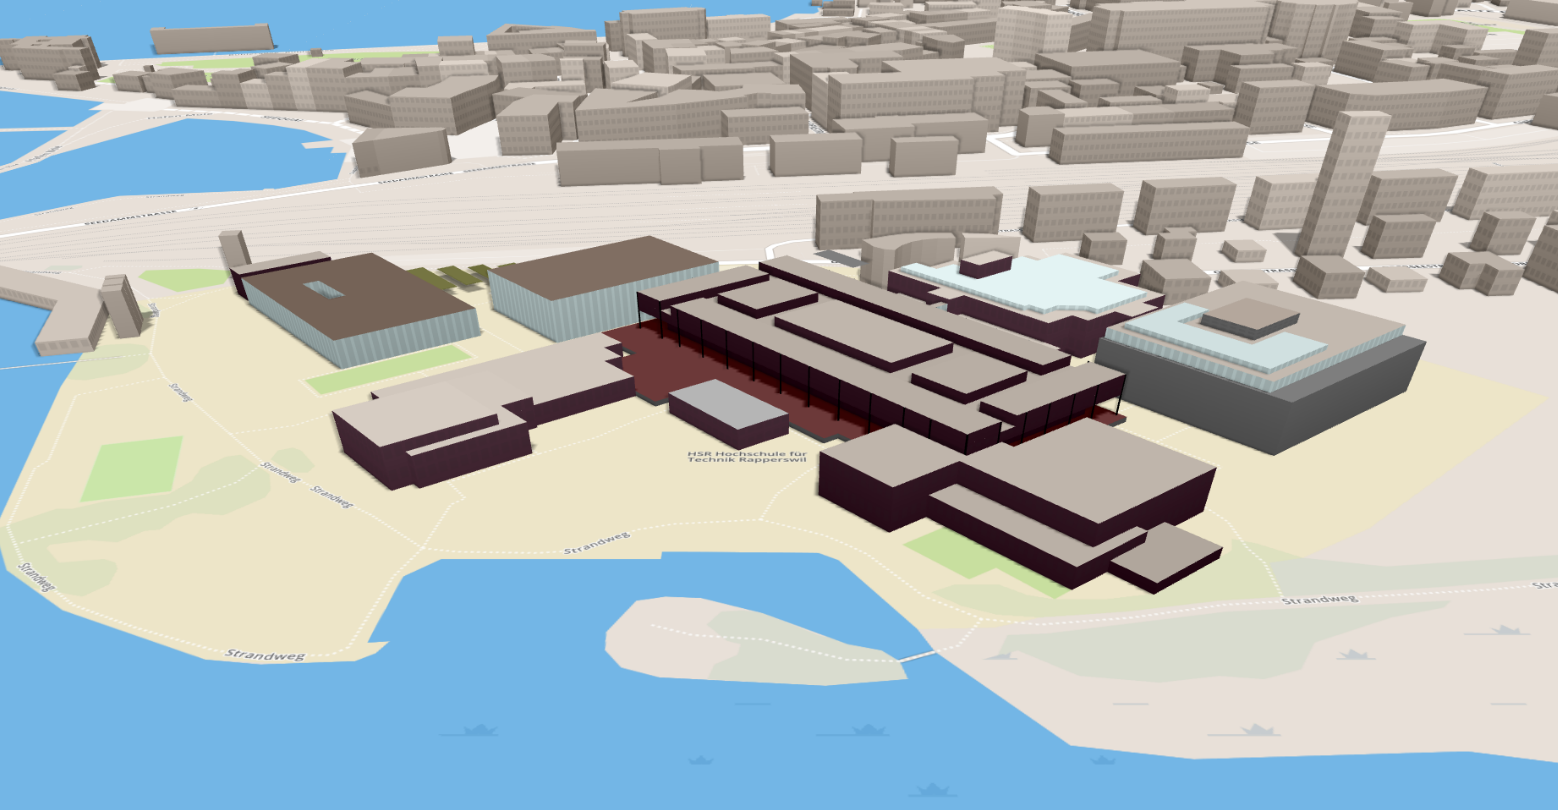
\includegraphics[width=1.0\textwidth]{images/routing/topology_example.png}
	\caption{Topologische Ansicht des Campus HSR}
	\label{fig:campus-hsr}
\end{figure}

\subsection{Das Zonen Model}
Um Kollisionen mit statischen Objekten zu vermeiden und sichere Flugwege zu erhalten, wurde ein Zonen Model eingeführt. Dieses ermöglicht dem Anbieter zu definieren, wo geflogen werden kann und wie hoch dort geflogen werden muss. Die Abbildung \ref{fig:demo-project} zeigt die Benutzeroberfläche für die Zonendefinition anhand des HSR-Campus.

\begin{figure}[H]
	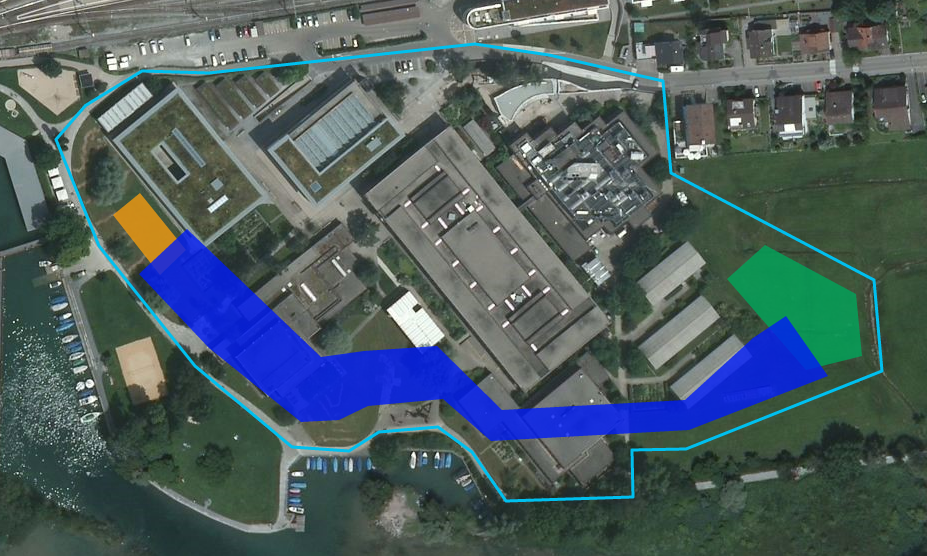
\includegraphics[width=1.0\textwidth]{images/routing/simpleProject_example.png}
	\caption{Verschiedene Flugzonen am Beispiel der HSR}
	\label{fig:demo-project}
\end{figure}
Jedes Polygon bildet eine Zone ab. Jede Zone enthält eine Flughöhe sowie einen Typ:
\begin{itemize}
	\item{\textbf{Order Zone:} Zone in welchem die Produkte des Projekts bestellt werden können. (\textit{hell blauer Rahmen})}
	\item{\textbf{Loading Zone:} Zone in welcher die Drohne beladen wird. (\textit{orange})}
	\item{\textbf{Delivery Zone:} Zone in der geliefert und geflogen werden darf. (\textit{grün})}
	\item{\textbf{Flight Zone:} Zone in der nur geflogen aber nicht geliefert werden darf. (\textit{blau})}
\end{itemize}

\subsection{Von der Zone zum Graphen}
Normalerweise wird eine Routenberechnung mit Hilfe eines Graphen durchgeführt, der durch die möglichen Wege (z.B. Strassen) definiert ist \cite{graph-routing}. Da die Zonen aber eine Fläche bilden, mussten diese zuerst in einen Graphen umgewandelt werden. \\

Folgende Lösungsmöglichkeiten wurden evaluiert:

\subsubsection{Erstes Konzept: Direkte Route}
Dieses Konzept umfasste den Ansatz den Start und den Endpunkt direkt zu verbinden, und bei einem Verlassen des Polygons dem Rand zu folgen (siehe Abb. \ref{fig:first-concet-routing}).

\begin{figure}[H]
	\centering
	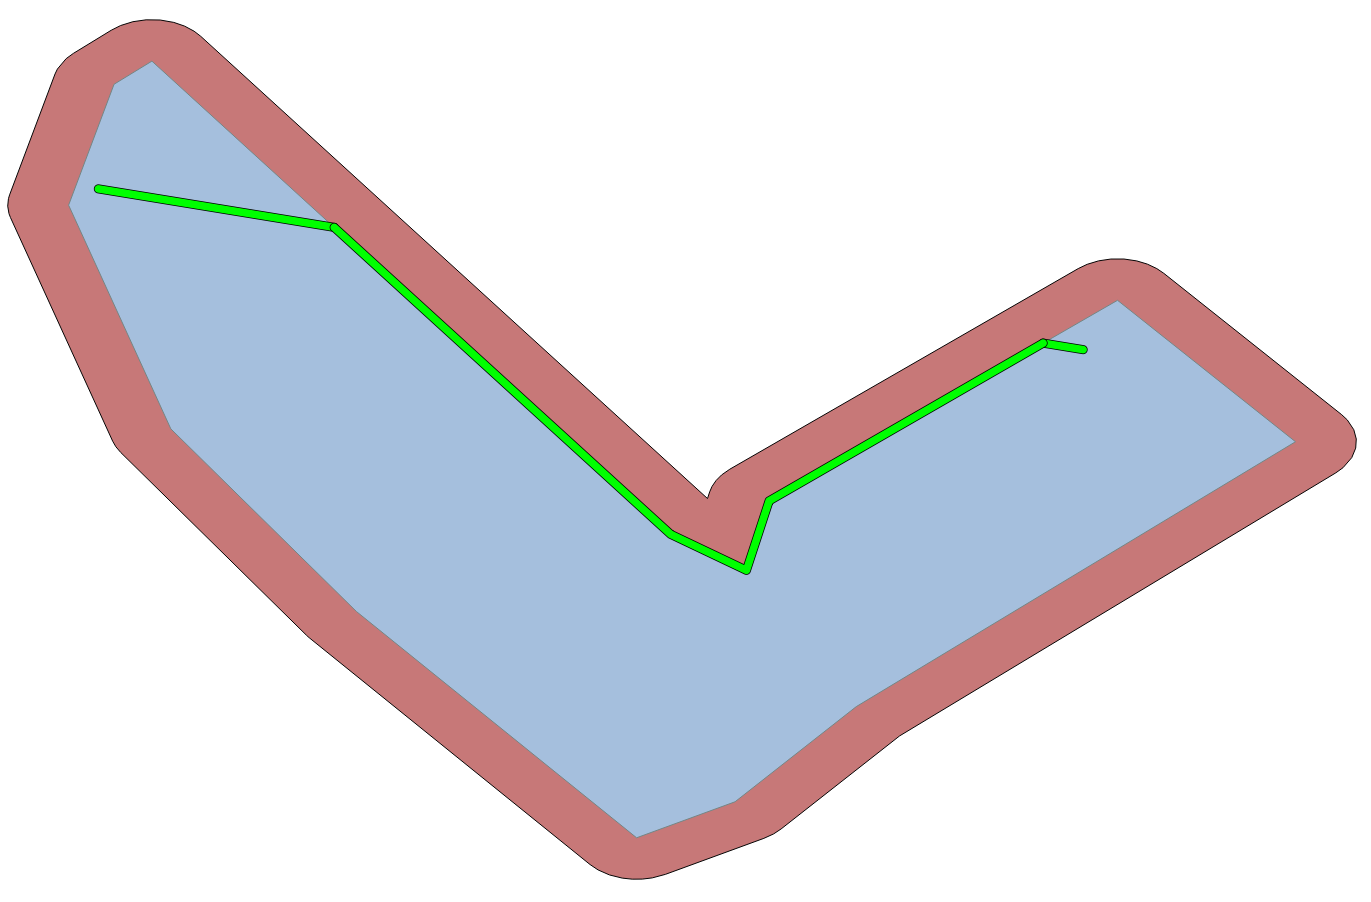
\includegraphics[width=0.8\textwidth]{images/routing/firstSolution.png}
	\caption{Erstes Konzept}
	\label{fig:first-concet-routing}
\end{figure}
Es wurde ausserdem ein Rand (\textit{Rot}) hinzugefügt. Diese Massnahme wurde getroffen, um allfällige GPS Ungenauigkeiten zu berücksichtigen.\\

Der Nachteil dieser Lösung zeigt sich bei grösseren Polygonen, wo unnötigerweise dem Rand entlang geflogen wird, obwohl ein Flug durch die Mitte viel sicherer wäre.
\newpage
\subsubsection{Zweites Konzept: Visibility Graph}
Das nächste Konzept orientiert sich an einem 'Visibility Graphen'. 
\cite[]{IEEEPaper} 

\blockquote{Using visibility graphs for determining the shortest path is very practical and intuitive. The visibility graph of a set of nonintersecting polygonal obstacles in the plane is an undirected graph whose vertices are the vertices of the obstacles and whose edges are pairs of vertices such that the open line segment between each two vertices does not intersect any of the obstacles.}

In unserem Fall haben wir den Gedanken umgedreht. Wir haben den Graphen in einem Polygon mit potentiellen Löchern berechnet. Diese Löcher stellen Enklaven für Bäume oder Gebäude dar. Das Konzept ist aber identisch, angewendet auf unser Beispiel Polygon ergibt sich folgende Abstraktion:
\begin{figure}[H]
	\centering
	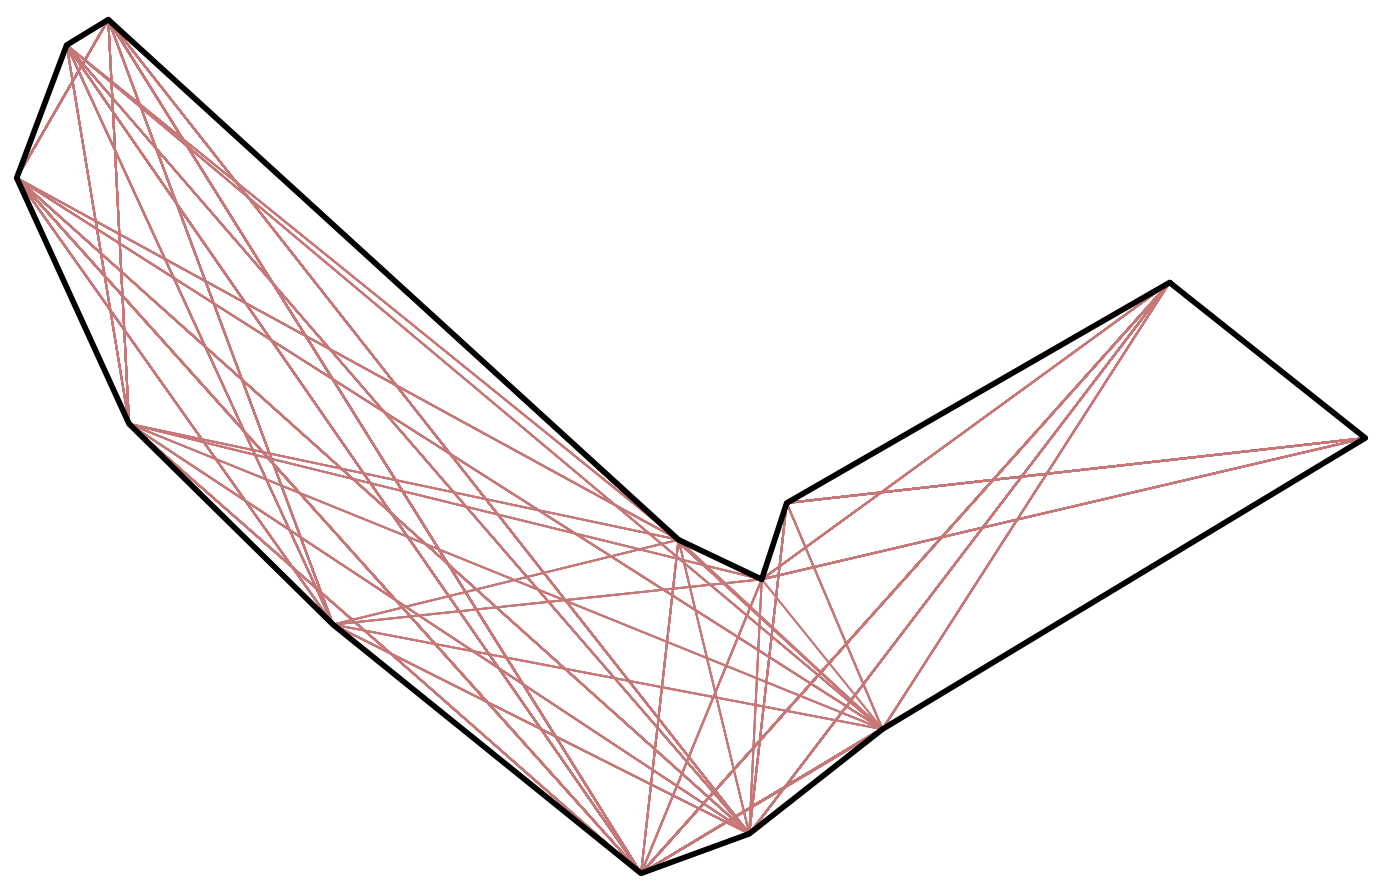
\includegraphics[width=0.8\textwidth]{images/routing/visibilityGraph.png}
	\caption{Visibility Graph in einer Flugzone}
	\label{fig:visibility-graph}
\end{figure}
Wie in der Abbildung \ref{fig:visibility-graph} gezeigt wird, verlaufen deutlich weniger Flugrouten entlang der Kante des Polygons. \\
Dies ist eine deutliche Verbesserung gegenüber dem ersten Konzept. Der Nachteil ist, dass die innere Ecke des L-förmigen Polygons sicher angeflogen wird, da es die vermeintlich kürzeste Route in einem nächsten Schritt darstellen würde. Aus diesem Grund haben wir uns gegen den Einsatz dieses Konzepts entschieden.\\

\subsubsection{Drittes Konzept: Straight Skeleton}
Da die Pfadfindung von \Gls{UAV} bereits ein weit erarbeitetes und erforschtes Gebiet ist, waren wir der Überzeugung, dass bereits verwendete Konzepte vereinfacht und abstrahiert werden konnten, um unser Problem zu lösen. Während vollständig autonome Drohnen an Hindernissen vorbei navigieren müssen, können wir uns auf einen bestehenden Flugkorridor verlassen.
\blockquote{The idea behind this method is to assign a function similar to the electrostatic potential to each obstacle and then derive the topological structure of the free space in the form of minimum potential valleys. The robot is positioned at the start point, and then the goal generates a strong attractive force. By the action of the force, the robot moves along the steepest descent of the potential to the goal, at the same time the obstacle generates a repulsive force to keep robot away from colliding with them} 

Die Kernaussage des zitierten Papers \cite[]{SkeletonUAV} ist, dass ein Pfad den grösstmöglichen Abstand zu den Hindernissen aufweisen soll. Auf unseren Fall übertragen, sind die Polygonränder die Hindernisse. Somit muss gewährleistet werden, dass die Drohne den grössten Abstand zu den Rändern aufweist. Aus diesem Grund erscheint diese Lösung für uns sehr geeignet, da sie mittenbetonte Routen vorschlägt. \\
\begin{figure}[H]
	\centering
	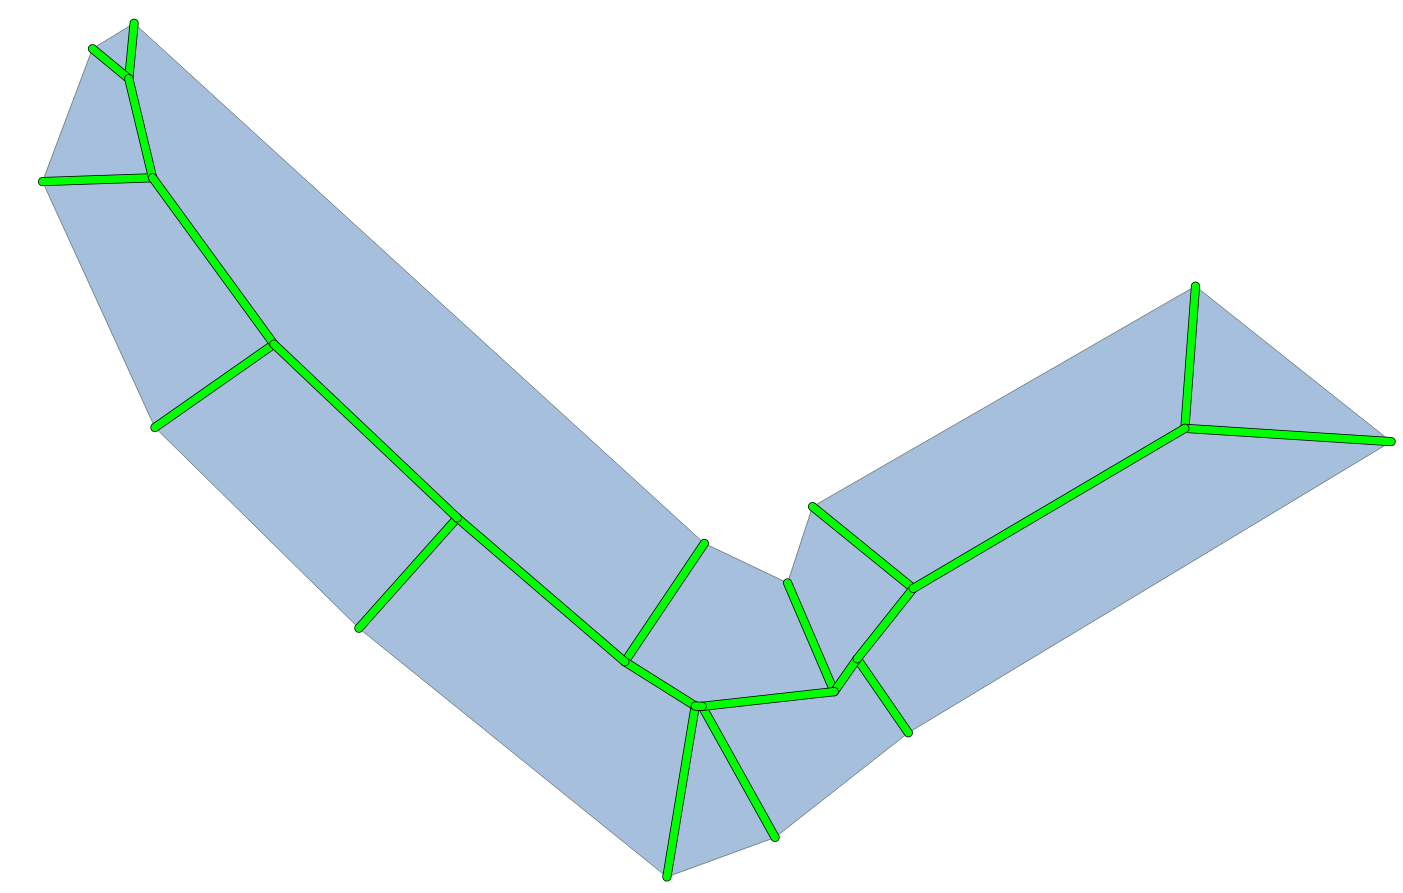
\includegraphics[width=0.8\textwidth]{images/routing/skeleton.png}
	\caption{Skeleton in Polygon}
	\label{fig:skeleton-in-polygon}
\end{figure}
Die Abbildung \ref{fig:skeleton-in-polygon} illustriert die Lösung mithilfe eines Skeletons. Dieses Konzept kann nachvollzogen werden, indem man sich das Polygon 3-dimensional vorstellt und dann  von der Mitte aus, parallel zu den Kanten schneidet. Der entstandene Grat ist hier als Linie sichtbar und wird als Skeleton bezeichnet. Der Felkel-Algorithmus, welcher diesen Skeleton aus einem 2-dimensionalen Polygon berechnet ist bereits in \Gls{CGAL} implementiert \cite{SkeletonCGAL} und war uns im weiteren Verlauf des Projektes von grossem Nutzen.\\






\subsection{Routing Algorithmus}
Nach der Herleitung des Graphen aus den Zonen, musste nun der passende Algorithmus gefunden werden, um einen möglichst effizienten Weg von A nach B zu finden. Es kamen vier Algorithmen in Frage, wobei ein Algorithmus sich als besonders geeignet herausstellte.
\begin{itemize}
	\item{\textbf{BFS:} (\textit{Breadth-first search}) Die Breitensuche durchsucht einen Baum in der Breite. Sie bringt garantiert eine Lösung, wenn eine Lösung vorhanden ist und kann problemlos mit Zyklen im Graph umgehen. Bei der Lösung handelt es sich aber nicht um die 'optimale Lösung' (kürzester Pfad). Die Lösung liefert den Pfad mit den wenigsten Knoten. \cite{AiClass}}
	\item{\textbf{DFS:} (\textit{Depth-first search}) Die Tiefensuche fängt an einem Knoten an und arbeitet sich dann in die Tiefe. Das Problem ist, dass sie sehr anfällig auf Zyklen ist und ohne weitere Hilfsmittel (loop detection oder pruning) nicht terminieren kann. \cite{AiClass}}
	\item{\textbf{A-Star:} Der A-Star Algorithmus arbeitet mit einer Heuristik und funktioniert effizienter als die zwei bereits genannten Algorithmen. Allerdings ist der Aufwand für die Umsetzung deutlich höher. \cite{AiClass}}
	\item{\textbf{Dijkstra:} Der Dijkstra-Algorithmus ist einer der bekanntesten Algorithmen in diesem Bereich. Der Vorteil ist, dass er grundsätzlich ohne Heuristik auskommt und robust mit Zyklen umgehen kann. Ausserdem können die Kanten mit einem Gewicht versehen werden und dadurch, der kürzeste Weg berechnet werden.}
\end{itemize}
Wir haben uns für den Dijkstra Algorithmus entschieden. Er liefert ohne Metrik eine ähnliche Lösung wie die BFS-Suche, kann aber im Nachhinein erweitert werden um effizientere Routen zu liefern.

\subsection{Höhenhandling}
Damit die Route 2-Dimensional berechnet werden kann, werden die Höhen erst zum Schluss berücksichtigt. Das Höhenhandling bildet den abschliessenden Schritt bei der Berechnung einer Route und wird in zwei Schritten durchgeführt:

\begin{itemize}
	\item{\textbf{Eindeutigkeit der Höhe:} In einem ersten Schritt werden die Zonen nach Höhe absteigend sortiert und Überlagerungen zugunsten der höheren Zone entfernt.}
	\item{\textbf{Einfügen von Schnittpunkten} An jedem Schnittpunkt des Pfads mit der Kante eines Polygons, wird ein Punkt eingefügt und mit der jeweiligen Zonenhöhe versehen.}
\end{itemize}
\begin{figure}[h]
	\centering
	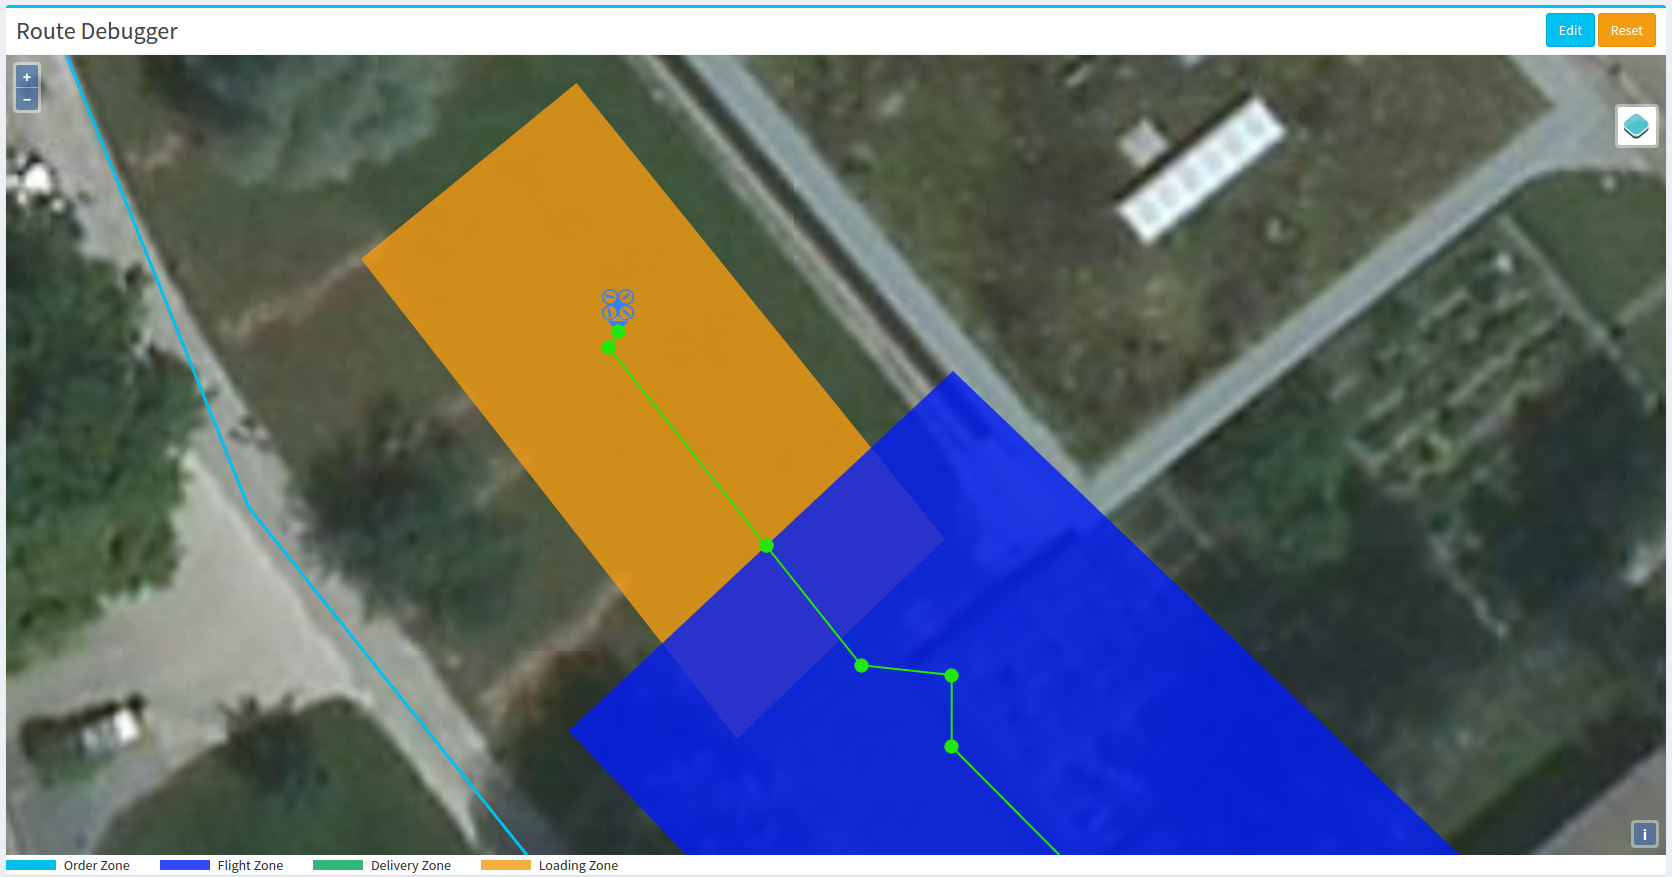
\includegraphics[width=1.0\textwidth]{images/routing/height_example.png}
	\caption{Beispiel der Höhe am Übergang zweier Polygone}
	\label{fig:polygon-border-example}
\end{figure}
Wie gemäss der Abbildung \ref{fig:polygon-border-example} ersichtlich ist, wird auf dem Übergang zwischen zwei Zonen ein Punkt eingefügt der für die Höhenänderung verwendet wird.
\newpage
\subsection{Wahl der Rückroute}

Der berechnete Pfad wird invertiert und bis auf den Abwurfpunkt am Ende der Route eingefügt. So ist garantiert, dass die Drohne auf dem gleichen Weg zurückfliegt.
